\documentclass{scrartcl}
\usepackage[latin1]{inputenc}
\usepackage[T1]{fontenc}
\usepackage{url}
\usepackage{graphicx}
\usepackage{ae}


\title{Documentation for Law Leecher}
\subtitle{Documentation for version 1.1}
\author{Tobias Vogel}
\date{\today}
\begin{document}

\maketitle

\begin{abstract}
This documentation describes propose, installation and usage hints as well as implementation details for \textit{Law Leecher}, in this order. The implementation part is intended to be read by programmers.

\textit{Law Leecher} is published under the 3-clause BSD license.\footnote{\url{http://en.wikipedia.org/wiki/BSD_licenses#Terms}}
\end{abstract}


\tableofcontents

\section{Propose}
In the late year 2007, an assistant of Professor Goetz came up with the task to read out some data from the Prelex\footnote{\url{http://ec.europa.eu/prelex/apcnet.cfm?CL=en}} database website which deals with \textit{Monitoring of the decision-making process between institutions}. In the database, meta information of the progress of European laws is stored. He needed some selected pieces of information, for example the legal basis, the primarily responsible or the steps the law took toward resolution. All this information had to be read out and put into a CSV file to process it further with a statistics program.

I wrote a tool to fulfill that. I chose Ruby\footnote{\url{http://www.ruby-lang.org/}} because it provided native regex support and the Interactive Ruby console to ensure a fast progress in development. And to learn something about Ruby in practice.

Moreover, the tool had to provide a graphical user interface (GUI) and had to be started quite easily without too much dependencies to the platform. For more details, see section~\ref{Deployment}.



\section{Installation and Usage}
\subsection{Installation}
It's quite easy to set up the program. Just follow these steps for installing it on Windows~XP.
\begin{enumerate}
  \item First, you have to install Ruby to be able to run the program. So, download it from \url{http://rubyinstaller.rubyforge.org/}. There is a One-Click Ruby Installer which makes installation very easy. I used Ruby in version 1.8.6 whose installer is available under \url{http://rubyforge.org/frs/download.php/29263/ruby186-26.exe}. Probably there are newer versions available in the meanwhile it should also work on. But you can always take version 1.8.6.
  
  Install it under the proposed directory, \texttt{c:\textbackslash ruby}. I will presume, you did so. You may follow the wizard's proposals for all other options.

  \item Second, install the toolkit which provides the GUI. It's named \textit{GTK}. ActiveState provides it under \url{http://www.activestate.com/store/download.aspx?prdGUID=f0cd6399-fefb-466e-ba17-220dcd6f4078} under the name \textit{ActiveTcl}. You have to download the package in version 8.4.18.0. The newer version 8.5.1.0 didn't work on my computer. If they didn't change it, you can use this direct download adress: \url{http://downloads.activestate.com/ActiveTcl/Windows/8.4.18/ActiveTcl8.4.18.0.284097-win32-ix86-threaded.exe}.
  
  Install it by double clicking on the executable you just downloaded. In the installation wizard, it finds out the location of the Ruby installation (\texttt{c:\textbackslash ruby}), however, I had two small boxes behind the path. I deleted them always I installed the system and I advise you to do the same. You may follow the wizard's proposals for all other options.


  \item Third, start the program by double clicking on \texttt{start.bat}. You can also double click on \texttt{main.rb}. Next to a black console window the following GUI should appear, shown in Figure~\ref{GUI}.
\end{enumerate}

  \begin{figure}[ht]
  \begin{center}
  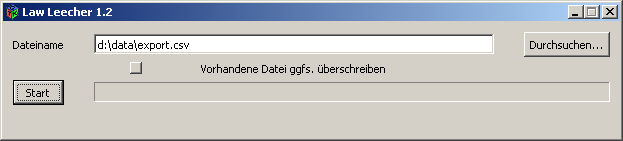
\includegraphics[width = \textwidth]{GUI.png}
  \caption{The graphical user interface of the program}
  \label{GUI}
  \end{center}
  \end{figure}



\subsection{Usage}
In the input area, type in the path and the file name of the output file. You can use the button on the right to select it by browsing over the file system. Check the check box under the input to overwrite a possibly existing file. You will get an error message in advance of starting the process, if a file exists there and you didn't check the check box. Press the start button to start the process. The progress bar will successively be filled. Below, a text will appear indication that the process has been completed.





\section{Implementation Details}
This section will describe the architecture of the program and point out some especially important aspects. It's intended for programmers who want to understand or to develop the program further. IBM NetBeans is a good IDE to program with.



\subsection{Architecture}
Figure~\ref{Architecture} draws a coarse-grained picture of the program.
\clearpage

  \begin{figure}[ht]
  \begin{center}
  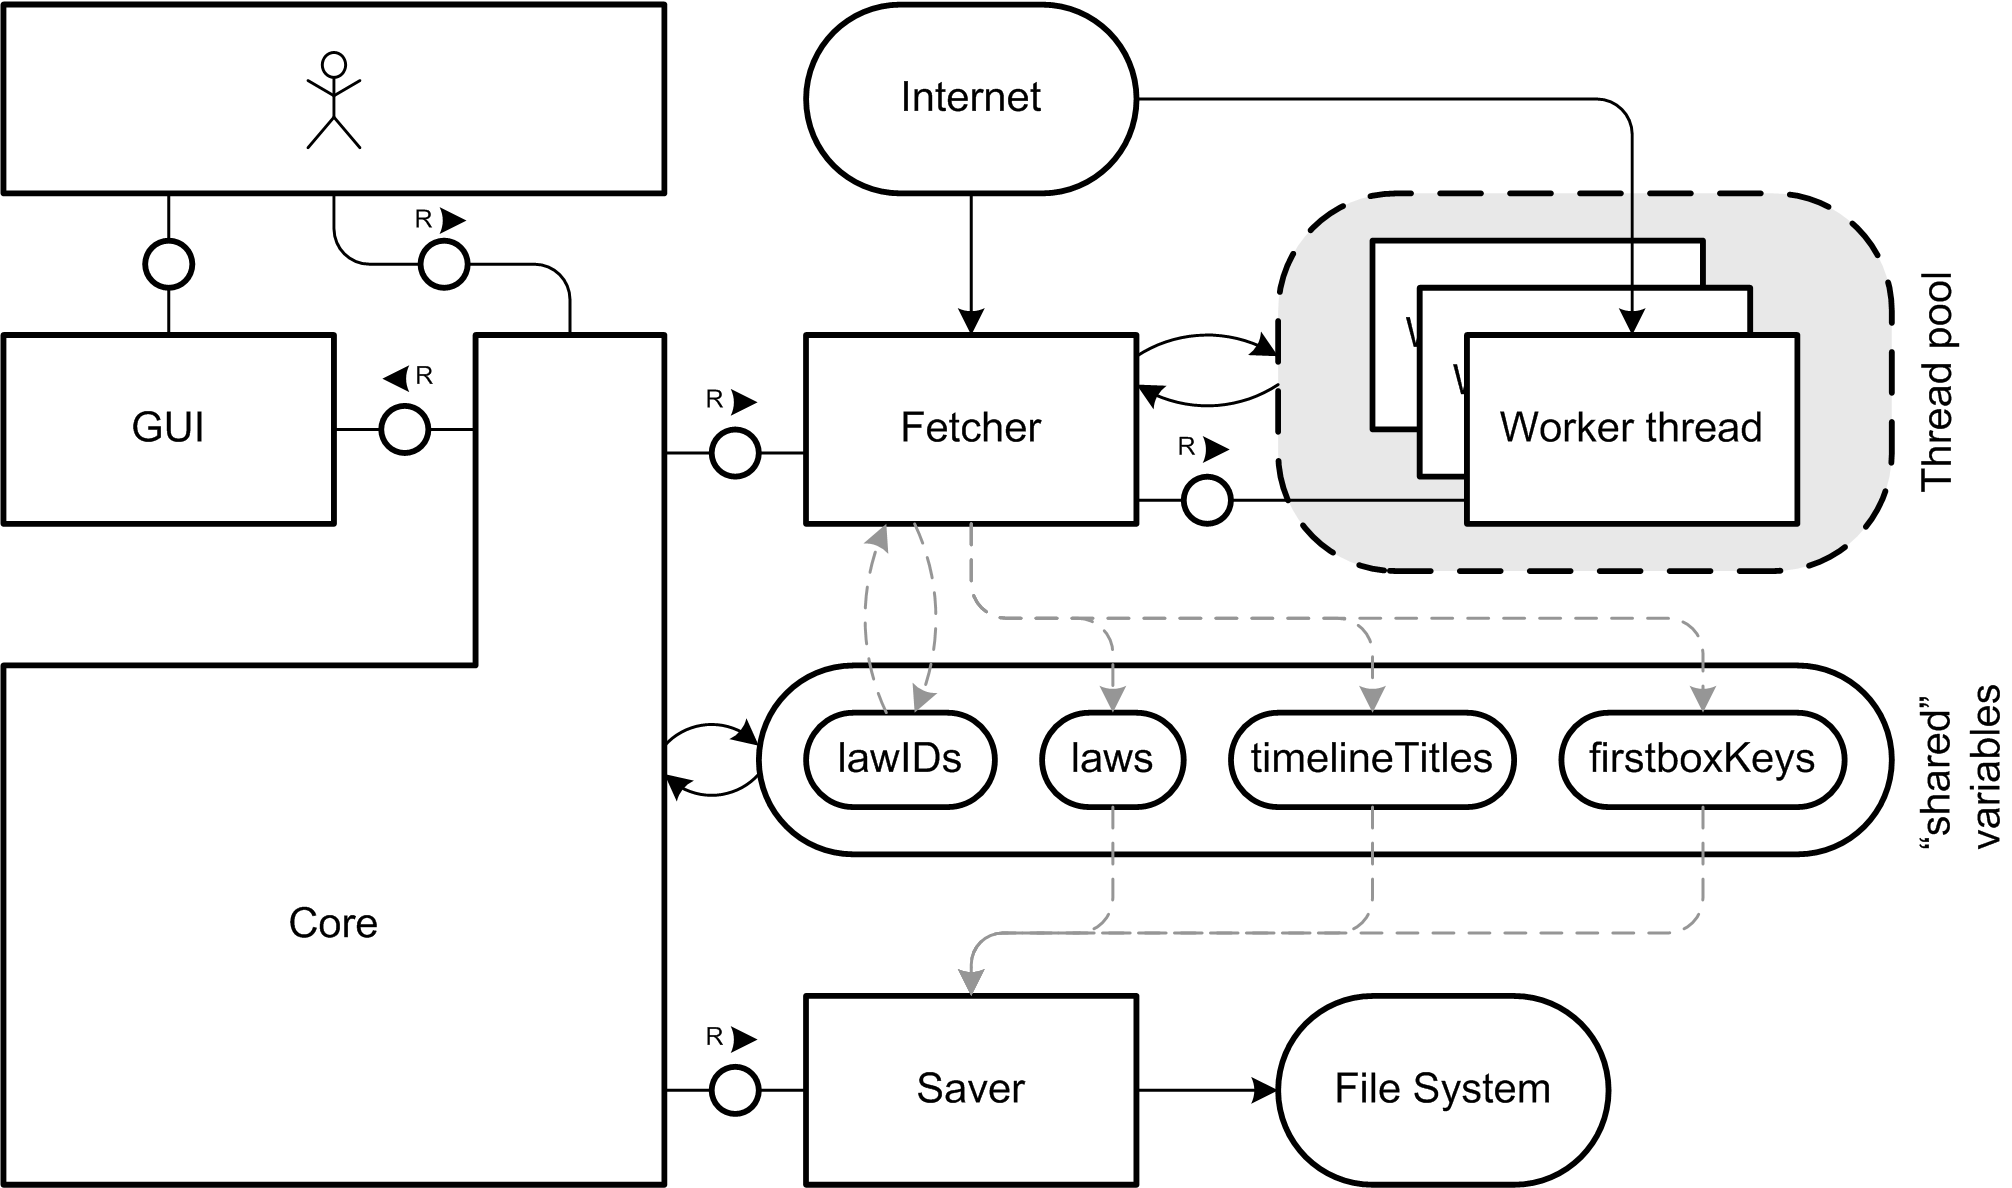
\includegraphics[width = \textwidth]{Architecture.png}
  \caption{The basic architecture of the program}
  \label{Architecture}
  \end{center}
  \end{figure}

The user starts the program (core) which controlls all components and additionally enables the user to communicate with the program via the GUI. The program's task is quite easy, so there are only two other agents: the Fetcher and the Saver, getting the information from the website (the Internet) respectively saving the gathered information in the output file. The main work is done within the Fetcher. Array:results is colored because it will be explained in more detail later on. The GUI variables correspond to the widgets.

Each agent is implemented within a class of the same name. The starting method is located within \texttt{main.rb}, which is no class. In the following, the classes and their main structure will be explained.



\subsubsection{Class \texttt{Core}}
The Core initializes the Fetcher and the Saver with pointers to the Core instance. The Core itself gets a pointer to the GUI instance (from the main method). Thus, the Core as well as Fetcher and Saver are enabled to do callbacks to the GUI which are needed for updating the GUI widgets. These callbacks are encapsulated by the Core within the \texttt{callback()} method. Therefore, they need the Core pointer.

Further, the Core handles the whole process of getting the information from the Fetcher and advising the Saver to save it. This handling is done in the \texttt{startProcess()} method.



\subsubsection{Class \texttt{Fetcher}}
The Fetcher is the most important agent. It basically does two tasks. First, it finds all law ids. Second, it grabs all required information for each law found in step one. The first is done within the \texttt{retrieveLawIDs()} method. The Fetcher sends a HTTP post request to the website. Instead of asking for 20 laws (like one does manually in the browser), it asks for 1,000,000 to suppress pagination\footnote{Currently, about 28,000 laws are contained in the data base}. The response is checked for validity (that there is really no pagination) and all law ids are crawled out and returned. Figure~\ref{Website} shows a screen shot of one of these law pages. The pieces of information with can be read out directly are marked. Additionally, there are some things which have to be calculated, first.

  \begin{figure}[ht]
  \begin{center}
  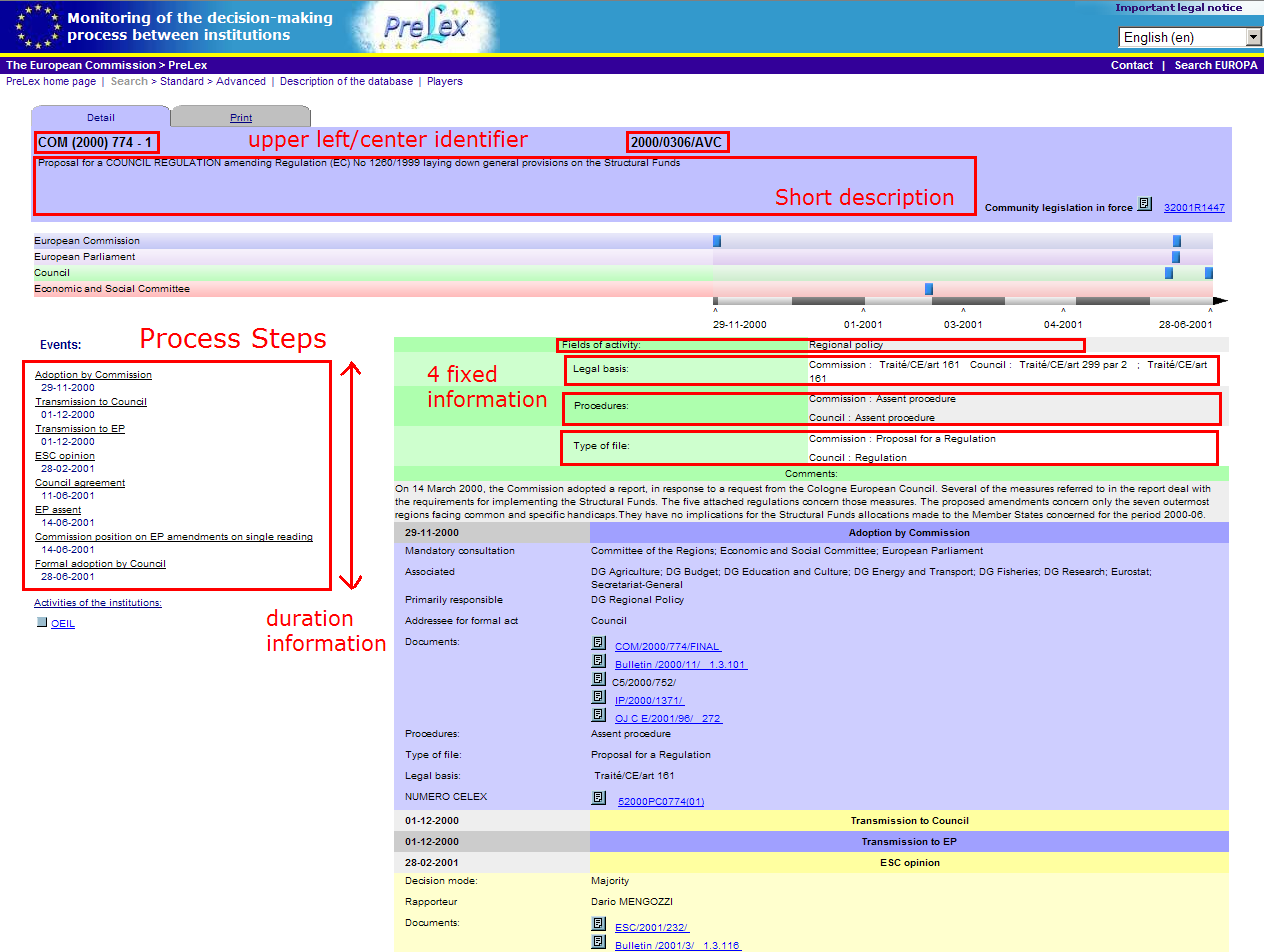
\includegraphics[width = \textwidth]{Website.png}
  \caption{The website and the pieces of information contained within}
  \label{Website}
  \end{center}
  \end{figure}


The \texttt{retrieveLawContents()} method executes a HTTP get request for each law (encapsulated within the \texttt{fetch()} method to consider the redirect which is made by the server). The data of the entries are collected via regular expressions. Since Ruby does not support lookbehinds\footnote{In version 1.9, Ruby allows lookbehinds, but not of arbitrary length, so it's not much better and I sticked to version 1.8.6.}, there are more or less always two very similar adjacent lines of regular expressions in the code.

Next to the information on the main area of the website there are process steps on the left. They record everything which happened to the law from the initial creation to the resolution or to discarding the law. Some steps may occur multiple times and there is no process step which occurs at every law. What's needed is the duration of each process step as difference to the first step measured in days. If there exists a process step named \textit{Adoption by Commission}, all earlier process steps for this law have to be ignored. If there is a process step named \textit{Signature by EP and Council}, additionally to the difference in days, the actual date of this step has to be saved. Process steps which occur multiple times in one law have to be saved in a way, that they are distinguishable. It is done by appending capital letters to the step names. Additionally, the duration for processing each law is temporarily stored. It is not saved in the output file but used for a short statistical calculation at the end of the program.

The information for each law is saved in a hash. The key is the process step or the category on the website, the value the corresponding entry respectively the date or the difference in days. Each hash is saved in an array, in turn. This array is returned by \texttt{retrieveLawContents()}. Additionally, a (mathematical) set containing all process steps is returned to getting knowledge about the table heads (next to the static information like legalBasis) without having to iterate again over all hashes to retrieve all keys.

Sometimes, the server does not respond in time. There are three or four errors who impersonate this. Then, the retrieving process for this law will be restarted. In case of other error types, the law is ignored.



\subsubsection{Class \texttt{Saver}}
The Saver simply saves the array of hashes in the output file with the given name. This is done in the \texttt{save()} method. First, the header containing the static fields and all (sorted) process steps is written to file. Afterwards, the entries, a law has, are written. Eventually, some statistical calculation is done and given to the user.

The Saver deals with Unicode, too. The text on the website is provided in Unicode. It has to be translated into ANSI (Latin-1), because Excel interprets CSV files in such way. This translation has been outsourced in the \texttt{convertUTF8ToANSI()} method which simply returns the converted string.



\subsubsection{Class \texttt{GUI}}
The GUI contains a description of all widgets in the window. It's programmed with GTK2. (See also section~\ref{Things to know}.) It also connects the widgets with the appropriate functions in the program.

The GUI is held responsive by implementing a cooperative multitasking. From time to time (more exact: at the beginning of each law processing via the \texttt{informUser()} method), the method \texttt{updateWidgets()} is called. The provided hash contains a bunch of information to update. That may be the progress bar or the status message. Afterward, a pending events handling loop is executed, allowing to move the window and to redraw the recently edited text.



\subsubsection{Class \texttt{Configuration}}
The Configuration class contains static constants and their getters which are used throughout the program. The year filter is more or less only for debugging reasons and has to be left an empty string to fetch all required laws.



\subsection{Data Model}
Figure~\ref{DataModel} shows, which information are saved about laws.
  \begin{figure}[ht]
  \begin{center}
  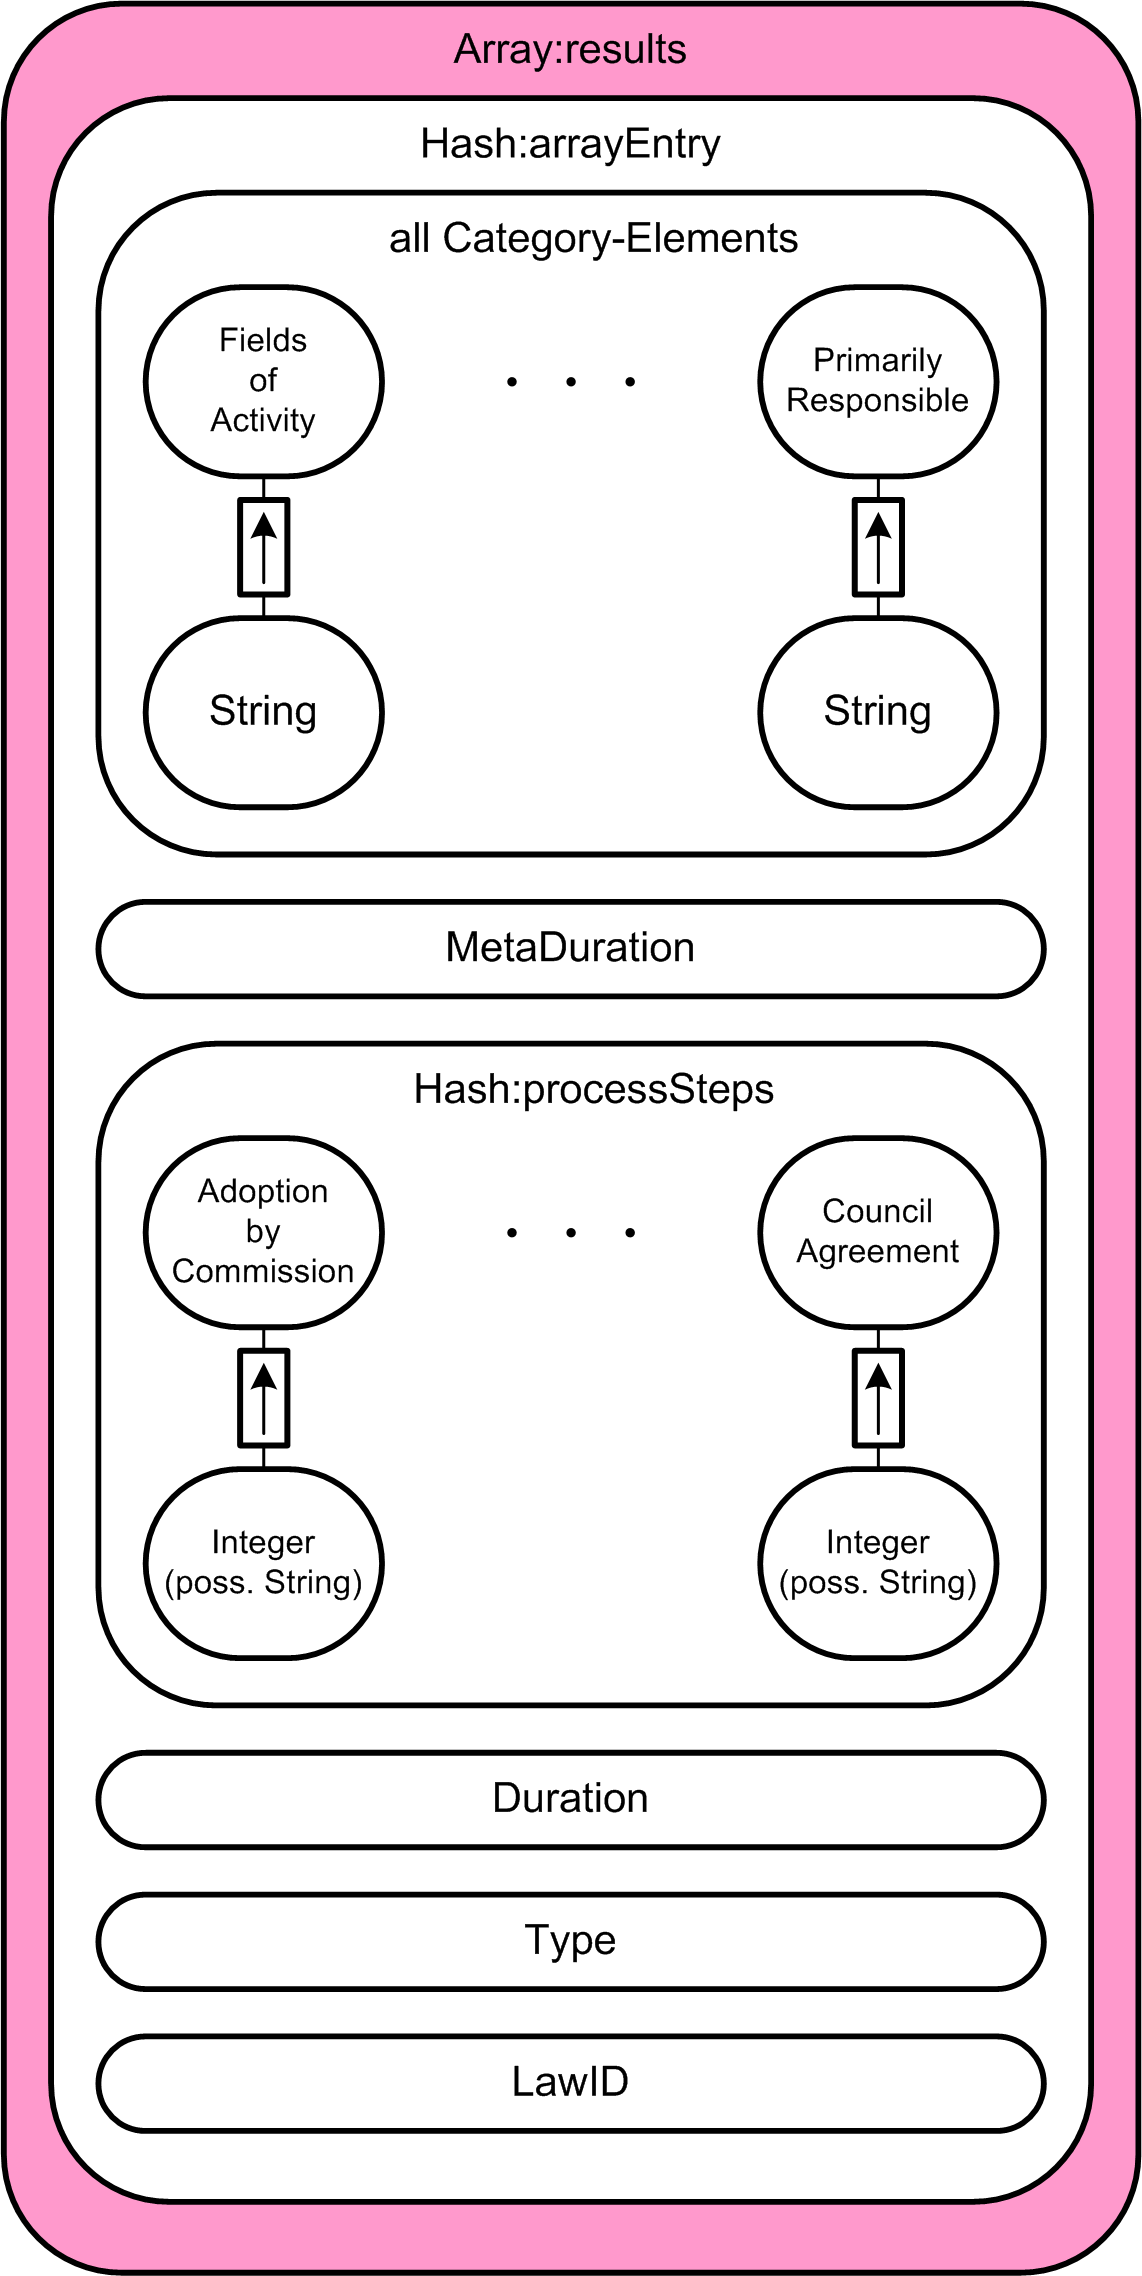
\includegraphics[width = 0.5 \textwidth]{Data_Model.png}
  \caption{The composition of the results array}
  \label{DataModel}
  \end{center}
  \end{figure}

The outer scope is the array of laws. Each law's information are saved within a hash. In a hash, the strings for the static categories are saved as well as the internal duration in milliseconds, the law's id and the law's type. The last entry is another hash, containing all the process steps of each law. There, only the actually occurring process steps are included. The value is either a date (for the first step resp. for \textit{Adoption by Commission} resp. for \textit{Signature by EP and Council}) or a duration in days.






\section{Further Things to Know}
\label{Things to know}
This section mentions some problems, I ran in and design decisions and explains them.


\subsection{Deployment}
\label{Deployment}
It would be desirable that the whole program could be started by a double click on one executable. Currently, you have to install Ruby and GTK(2) and to copy the Ruby source files to a directory and start \texttt{start.bat} or \texttt{main.rb}.
There is a possibility to create executables out of Ruby programs, called rubyscript2exe\footnote{\url{http://www.erikveen.dds.nl/rubyscript2exe/}}. It's available as Ruby Gem. Install it with the following command.
\begin{verbatim}
gem install rubyscript2exe
\end{verbatim}
Afterward, it is available via the rubyscript2exe command. You provide a Ruby file and the script transforms it and all dependent files into an executable.

However, it does not include external sources like icons or images or libraries. Thus, install the tar2rubyscript\footnote{\url{http://www.erikveen.dds.nl/tar2rubyscript/}} Gem with the following command.
\begin{verbatim}
gem install tar2rubyscript
\end{verbatim}

It converts a Ruby program including the required resources into a single Ruby file. With rubyscript2exe you can convert this into an executable.

Sadly, I didn't manage to get it to work with GTK. See also section~\ref{Toolkits}.



\subsection{Testing}
For testing, I created a file called Tester. NetBeans allows running and debugging single files, so it was just what I needed. The tester file was the following:

\begin{verbatim}
require 'core'
require 'g_u_i.rb'

core = Core.new
core.addGuiPointer(GUI.new(core))
fetcher = Fetcher.new(core)

lawsToDebug = [123456, 654321]

results, processStepNames = fetcher.retrieveLawContents(lawsToDebug)
Saver.new(core).save(results, processStepNames, "c:\\export.csv")
\end{verbatim}
The lawsToDebug array always contained the law ids from the laws which caused trouble.

Another way to test/debug was to add the year filter in the Configuration class and to use just the first types array entry (returning \texttt{@@types.first}).



\subsection{Toolkits}
\label{Toolkits}
I tried to use three different toolkits. First, I used Tcl/Tk\footnote{\url{http://home.arcor.de/scite/gui_tk.html}} which could be compiled to an executable, but wasn't easy to program with.

Then, I tried GTK2\footnote{\url{http://ruby-gnome2.sourceforge.jp/}}, which didn't compile (as I later learned), but which was easy to program. It provided a responsive GUI, a progress bar and a common file dialog.

Third, I found wxRuby\footnote{\url{http://wxruby.rubyforge.org/wiki/wiki.pl}} which could be compiled but was terrible to use. It didn't have a single progress bar. I didn't get far enough to say, whether it has a responsive GUI. Additionally, it's not that well documented.



\subsection{Possible Adjustments and Future Work}
There are some possibilities to improve the program. The approach to parse the website via regular expressions is a valid one. Perhaps the expressions can be optimized by making them shorter (esp. by lookbehinds, when they are working), using less regular expressions or by somehow preprocessing them, if this is possible. Further, leaving regular expressions out and use an XML parser instead, could reduce processing time. However, the web site currently does not validate. Furthermore, if the website changes, the regular expressions have to be touched.

Another approach could be to introduce multi threading into the program. The time, the program waits for the web server's answer could be used for scraping the contents of already-fetched pages. And maybe, also for multi processor systems, that would be advantageous.

Additionally, a correct internationalization would eliminate the German strings from the program code.

Currently, there is a hack to allow dates before 01.01.1970. If there is a process step before, a year offset of 10 years is set. The last entry is also decremented by these 10 years and so, the duration is calculated properly. It will not work, if laws exist before 01.01.1960.

Also, a \# must not occur in the scraped texts on the website, because it's the value divider for the CSV file.

The program won't stop running if the server can't be reached (e.g. if the computer is disconnected from the network). Perhaps this is not desirable and/or leads to memory problems.

\section{hinzufügen}
komplett gehts nicht mit jruby auf 2x2000, 4gb ram, mxm=2048, nogarbagecollectordings
sondern nur mit echtem ruby



\end{document}
